\chapter{React Native}
\label{ch2}


\section{Декларативний}
\label{section.2.1}

React спрощує створення інтерактивних інтерфейсів.
Вам потрібно лише описати, як різні частини інтерфейсу виглядають у кожному стані вашого додатку і React ефективно оновить та відрендерить лише потрібні компоненти.
Декларативні інтерфейси роблять наш код більш передбачуваним і його набагато легше налагоджувати.


\section{Заснований на компонентах}
\label{section.2.2}
React Native заснований на основі інкапсульованих компонентів, які керують власним станом, і з них будують складні інтерфейси.
Оскільки логіка компонентів написана на JavaScript, замість шаблонів, ми з легкістю можемo передавати складні дані у додатку і зберігати стан окремо від DOM.


\section{JSX}
\label{section.2.3}
Розглянемо оголошення змінної:
\begin{lstlisting}[style=light, language=Python,label={lst:jsx_hello},caption=JSX Hello World]
const element = <h1>Hello, world!</h1>;
\end{lstlisting}

Цей дивний синтаксис тегів не є ні рядком, ні HTML.

Він має назву JSX, і це розширення синтаксису для JavaScript.
Його використовує React, щоб описати інтерфейс користувача.
JSX може нагадувати мову шаблонів, але з усіма перевагами JavaScript.

React використовує той факт, що логіка виводу пов’язана з іншою логікою інтерфейсу користувача: як обробляються події, як змінюється стан з часом і як дані готуються для рендерингу.

Замість того, щоб штучно відокремити технології, розмістивши розмітку і логіку в окремих файлах, React розділяє відповідальність між вільно зв’язаними одиницями, що містять обидві технології і називаються "компонентами".
React не вимагає використання JSX, але більшість людей цінують його за візуальну допомогу при роботі з інтерфейсом користувача в коді JavaScript.
Він також дозволяє React показати зрозуміліші повідомлення про помилки та попередження.


\section{Система побудування Expo}
\label{section.2.4}
React Native пропонує два різних способи побудування проекту \textbf{«керований»} та \textbf{«простий»} робочими процесами.
\begin{itemize}
    \begin{item}
        За допомогою \textbf{керованого} робочого процесу ви пишете лише інструменти та служби JavaScript / TypeScript та Expo, які піклуються про все інше.
    \end{item}
    \begin{item}
        У \textbf{простому} робочому процесі ви маєте повний контроль над кожним аспектом власного проекту, а інструменти та послуги Expo трохи більш обмежені.
    \end{item}
\end{itemize}

В обох випадках використовується екосистема інструментів, що спрощують процес пободування проекту, ховаючи деталі та називається Expo.
Expo - платформа для універсальних додатків React, набір інструментів та служб, побудованих навколо React Native та власних платформ, які допомагають вам розробляти, будувати, розгортати та швидко переглядати iOS, Android та веб-додатки з тієї самої кодової бази JavaScript / TypeScript.\cite{expo_doc}


\section{Запити до мережі. Fetch API}
\label{section.2.5}
React Native надає API Fetch для ваших мережевих потреб.
API Fetch забезпечує інтерфейс для отримання ресурсів (у тому числі по всій мережі).
Буде здаватися звичним кожному, хто використовував XMLHttpRequest, але новий API забезпечує більш потужний та гнучкий набір функцій.
Fetch забезпечує загальне визначення Requestі Responseоб'єктів (та інших речей, пов'язаних із мережевими запитами).
Це дозволить їх використовувати там, де вони потрібні в майбутньому.

Fetch API залежить від Promise.
Promise або "обіцянка" - це проксі для значення, яке не обов'язково відомо при створенні об'єкту.\cite{promise_doc}
Інакше кажучи, це API обгортка, яка задає контракт згідно которого promise(обіцянка) може знаходитись в одному зі станів:
A Promise знаходиться в одному з таких станів:
\begin{itemize}
    \begin{item}
        \textbf{в очікуванні(peding)}: початковий стан, ні виконаний, ні відхилений.
    \end{item}
    \begin{item}
        \textbf{виконано(fulfilled)} : це означає, що операція була успішно завершена.
    \end{item}
    \begin{item}
        \textbf{відхилено(rejected)} : означає, що операція не вдалася.
    \end{item}
\end{itemize}

Прикладом коду, котрий виконує запит та отримує відповідь в форматі JSON можна знайти в додатку \ref{lst:rn_network}.


\section{Realm React Native}
\label{section.2.6}
В випадку вибору бази даних треба розглянути наступні фактори:
\begin{itemize}
    \begin{item}
        \textbf{Технологія:} з відкритим кодом чи власністю?
    \end{item}
    \begin{item}
        \textbf{Архітектура:} SQL або NoSQL?s
    \end{item}
    \begin{item}
        \textbf{Масштабованість:} чи ви будете самостійно розміщувати або скористаєтесь масштабованою послугою?
    \end{item}
\end{itemize}

Ринок надає можливість використання таких рішень як:

\begin{longtable}[c]{|l|l|l|}
    \caption{Порівняння Баз Даниx React Native}
    \label{tab:rn_db_comparison} \\
    \hline
    & Сирцевий код  & Тип реаліаційної БД \\ \hline
    \endhead
%
    Back4app        & Відкритий     & SQL, NoSQL          \\ \hline
    Cloud Firestore & Пропрієтарний & NoSQL               \\ \hline
    DigitalOcean    & Відкритий     & SQL                 \\ \hline
    AWS RDS         & Відкритий     & SQL                 \\ \hline
    Realm           & Відкритий     & NoSQL               \\ \hline
\end{longtable}

Під час роботи над тестовим продуктом було зроблене рішення використати Realm.
Рішення базувалося скоріше на потребах швидкого та простого в інтеграції рішення.
Як наведено в додатку \ref{lst:rn_realm}  конфігурація в цілому є дуже проста (також див. \ref{fig:rn_realm}).

Спочатку ми описуємо схему бази даних. В даному випадку одна таблиця.
Створюємо об'єкт конфігурації, котрий буде використаний, щоби відкрити підключення до бази даних.
Передавши конфігурацію ми отримаємо відкрите підключення до бази даних та робимо запит до таблиці.
Запит повертає нам результат зі збереженими даним з котрих ми робимо копію кожного об\'єкту.
Особливість Realm об\'єктів полягає в тому, що вони є вікном до курсору в таблиці.
Щоби уникнути випадкових змін в таблиці ми спеціально робимо копію, яка є "чистим" об\'єктом від\'єднаним від БД.

\begin{figure}
    \label{fig:rn_realm}
    \begin{center}
        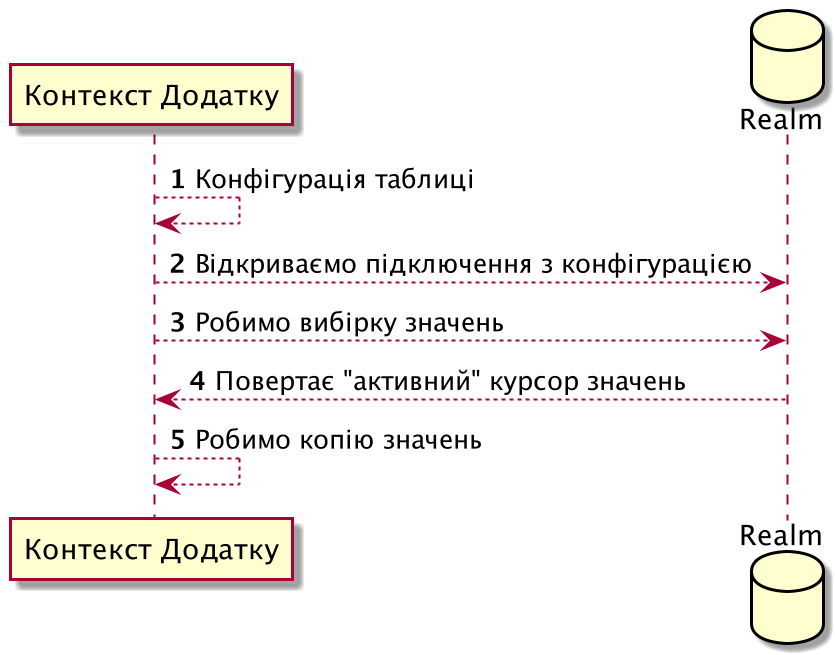
\includegraphics[scale=0.4]{rn_realm.png}
    \end{center}

    Взаємодія React Native додатку з БД
\end{figure}


\section{Управління станом в React Native}
\label{section.2.8}
React Native використовує систему звротніх викликів або так званих "хуків".
Наприклад, \textbf{useState} - це Хук, що дозволяє додавати стан React до функціональних компонентів.

"useState" оголошує "змінну стану" та повертає пару значень: поточний стан та функцію, яка його оновлює.
Наша змінна називається, data ми можемо називати її як завгодно, наприклад banana \ref{lst:rn_state_hooks}.

Використовуючи useEffect хук, ми повідомляємо React, що наш компонент повинен виконати додаткову фунцію після рендерингу.
React запам'ятає передану нами функцію (яку ми будемо називати "ефектом") і викличе її пізніше після оновлення UI нашого додатку.

Ефект котрий ми створили буде виконаний при ініціалізації додатку. І як результат виконання ми отримаємо дані з локальної бази які ми і відобразимо (див. на \ref{fig:rn_realm})).

\begin{figure}
    \begin{center}
        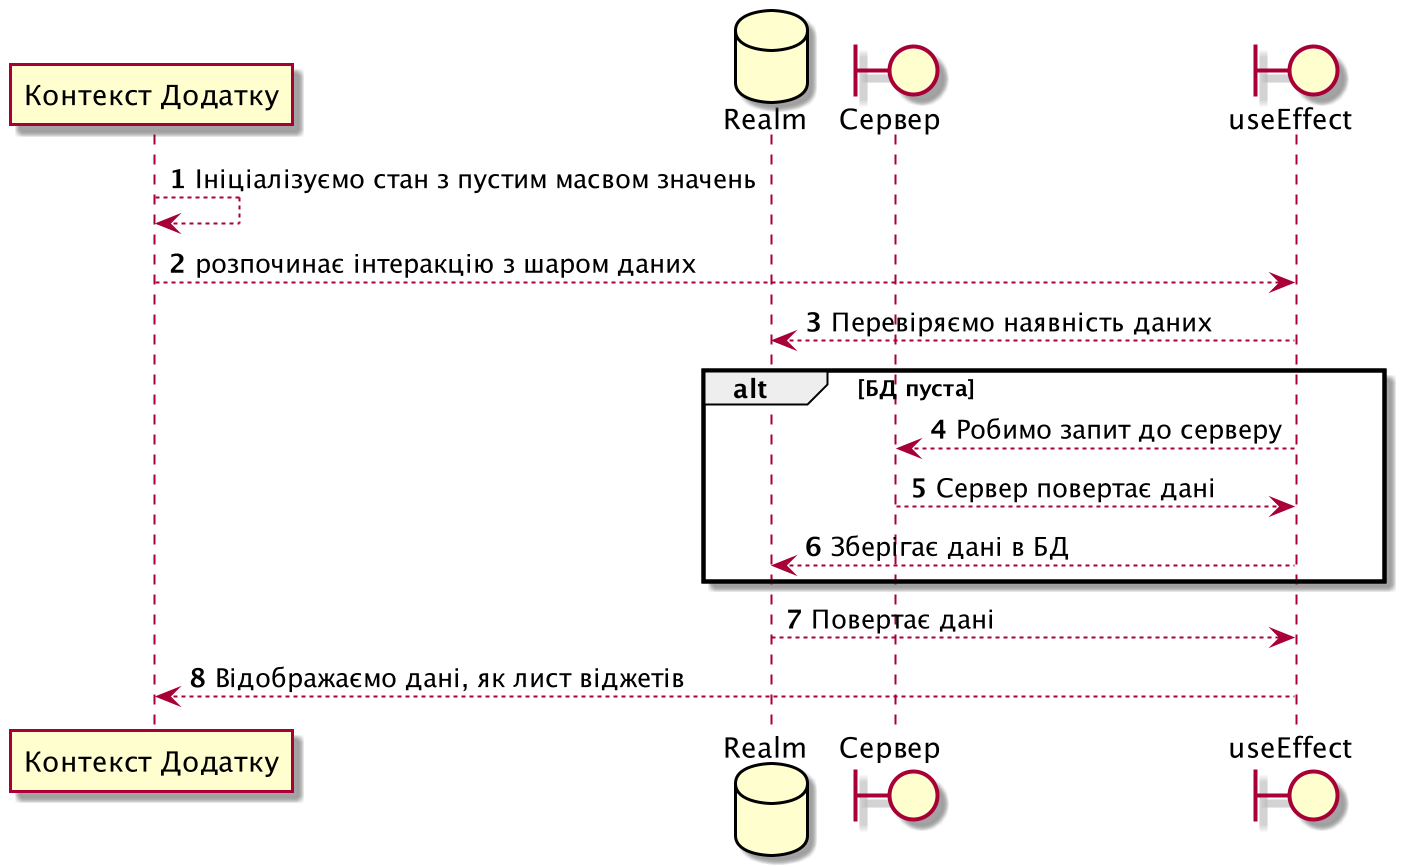
\includegraphics[scale=0.3]{app_widget.png}
        \caption{Схема послідовності віджету App та інтеракція з шаром даних}
        \label{fig:rn_realm}
    \end{center}
\end{figure}

Даний підхід дозволяє швидко і в простий спосіб сконфігурувати стан нашого компоненту.
Хоч це і звучить просто нажаль, в більш складних компонентах з великою кількістю взаємодій з користувачем такий підхід призведе до високої зв'язаності коду.
В свою чергу ми отримаємо складний до зрозуміння сирцевий код і нестабільне рішення з великою кількістю помилок.
Для рішення цієї проблеми можна застосувати архітектуру Redux.

Redux - передбачуваний контейнер стану для Javscript додатків Apps (див. на \ref{fig:rn_realm}))..
Redux допомагає писати програми, які поводяться послідовно , працюють у різних середовищах (клієнтських, серверних та власних) і легкі для перевірки. \cite{redux_home_page}
Централізація стану та логіки вашого додатка забезпечує потужні можливості, такі як скасування / повтор , стійкість стану та багато іншого. \cite{redux_home_page}

\begin{center}
    \begin{figure}
        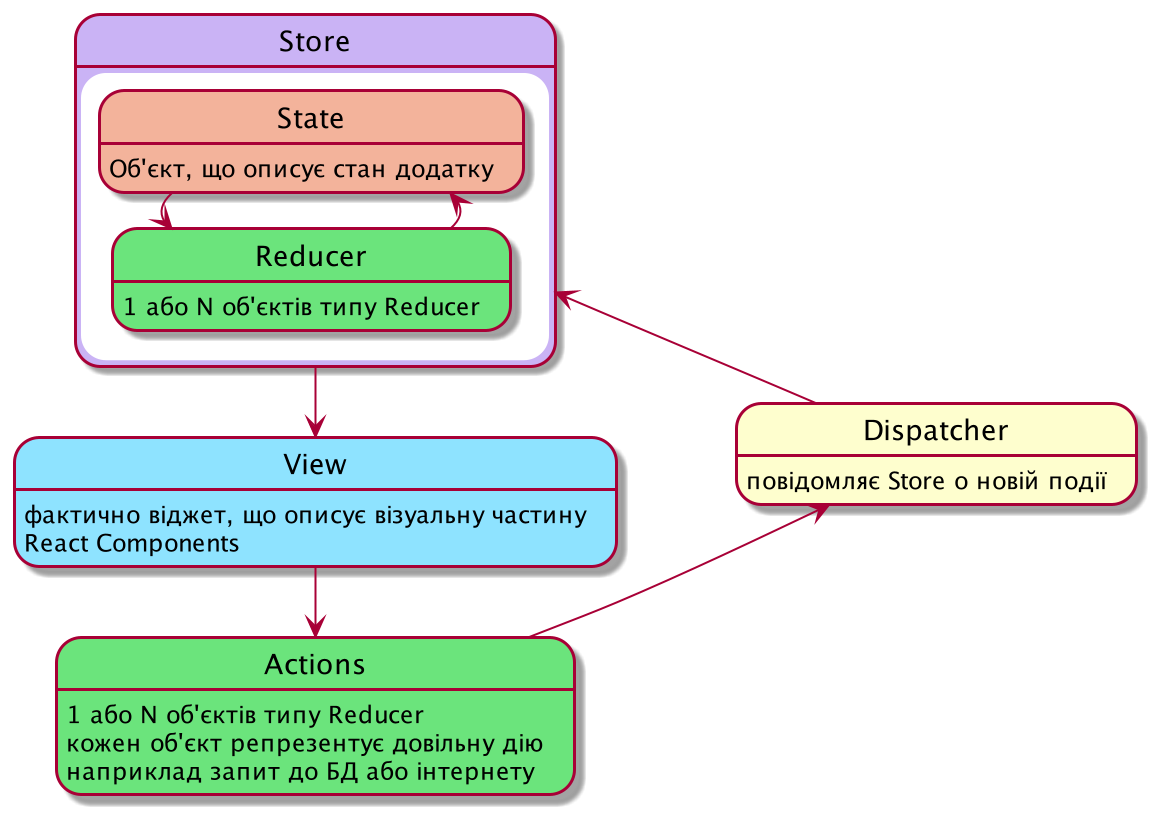
\includegraphics[scale=0.33]{redux.png}
        \caption{Схема Redux}
        \label{fig:rn_redux}
    \end{figure}
\end{center}


\section{Тестування в React Native}
\label{section.2.9}
У міру розширення вашої кодової бази невеликі помилки та крайні випадки, на які ви не очікуєте, можуть перетворюватися на більші збої.
Помилки призводять до поганого досвіду для користувачів і, зрештою, до втрат бізнесу.
Одним із способів полібшити якість сирцевого коду є написання тестів.

Одним з найкращих способів виправити помилку в коді є написання тесту, який виявляє її.
Потім, коли ви виправляєте помилку і повторно запускаєте тест, якщо він проходить, це означає, що помилка виправлена, і ніколи повторно не буде впроваджена в сирцевий код проекту.

Тести також можуть служити документацією для нових людей, які приєднуються до вашої команди.
Людям, які ніколи раніше не бачили кодової бази, аналіз тестів може допомогти зрозуміти, як працює існуючий код.
Нарешті, але не менш важливим є те, що більш автоматизоване тестування означає менше часу, проведеного за допомогою ручного контролю якості, звільняючи цінний час.

За замовчуванням React Native постачається з тестовою структурою Jest. \cite{jest_home_page}

\begin{lstlisting}[style=light, language=Python,label={lst:rn_jest_test},caption=Jest Unit Test]
  it('given 2 +2 returns 4', () => {
    expect(2 + 2).toBe('red');
  });
\end{lstlisting}

Jest дозволяє групувати тести з уживанням функцій "describe"(опис).
Підтримує хуки для ініціалізації стану "beforeEach"(перед кожним) та "beforeAll"(після всіх).

Unit test(єдносткові тести) допомагають протестувати тільки бізнес логіку.
Для тестування UI компонентів застосовується компонентне тестування.
Навіть якщо логіка вашого додатка має високий рівень охоплення тестуванням і є правильною,
без тестування компонентів ви все одно можете доставити непрацюючий інтерфейс для своїх користувачів.

Під час тестування компонентів React можна перевірити дві речі:

\begin{itemize}
    \begin{item}
        \textbf{Взаємодію:} для забезпечення належної поведінки компонента під час взаємодії з ним користувачем (наприклад, коли користувач натискає кнопку)
    \end{item}
    \begin{item}
        \textbf{Рендеринг:} щоб переконатися, що вихідний вигляд компонента, який використовує React, правильний (наприклад, зовнішній вигляд кнопки та розміщення її в інтерфейсі)
    \end{item}
\end{itemize}

Однак требу мати на увазі, що тестування компонентів - це лише тести JavaScript, що виконуються у середовищі Node.js.
Вони не беруть до уваги будь-який iOS, Android або інший код платформи, який підтримує компоненти React Native.
Звідси випливає, що вони не можуть надати вам 100\% впевненості, що все працює.
Якщо в коді платформи iOS або Android є помилка, вони її не знайдуть.

Останій клас тестів - це ті, що дозволяють протестувати в наскрізний спосіб наш додаток (далі E2E - End to End).
Це робиться шляхом запуску тестів на фінальній зборці додатку виконаному в середовищі Android або iOS.
У тестах E2E ви більше не думаєте про компоненти React, React Native API, Redux чи будь-яку бізнес-логіку.

Тести E2E дають вам максимально можливу впевненість у тому, що частина вашого додатка працює.
Однак в випадку E2E ми мусимо враховувати наступні компроміси.

\begin{itemize}
    \item їх написання займає більше часу порівняно з іншими типами тестів
    \item вони працюють повільніше
    \item вони більш нестабільні "flakky" ("flakky"  - це тест, який випадково проходить і не проходить без будь-яких змін в коді)
\end{itemize}

Доступно кілька інструментів тестування E2E.
\begin{itemize}
    \item у спільноті React Native Detox є популярним фреймворком, оскільки він спеціально підходить для додатків React Native.\cite{detox_home_page}
    \item ще однією популярною бібліотекою для iOS та Android додатків є Appium.\cite{appium_home_page}
\end{itemize}


\section{Структура проекту в React Native}
\label{section.2.10}

\begin{lstlisting}[style=light, language=Python,label={lst:rn_app_structure},caption=React Native App Layout]
├── App.js (1)
├── Readme.md
├── __tests__ (2)
│ └── App.js
├── android (3)
│ ├── app
│ ├── build
│ ├── build.gradle
│ ├── gradle
│ ├── gradle.properties
│ ├── gradlew
│ ├── gradlew.bat
│ ├── local.properties
│ └── settings.gradle
├── app.json (5)
├── babel.config.js (6)
├── index.js (7)
├── ios (4)
│ ├── BreedRN
│ ├── BreedRN.xcodeproj
│ ├── BreedRN.xcworkspace
│ ├── Podfile
│ ├── Podfile.lock
│ └── Pods
├── metro.config.js (8)
├── node_modules (11)
├── package-lock.json (10)
└── package.json (9)
\end{lstlisting}

\begin{enumerate}
    \item \textbf{App.js} сирцевий код нашого додатку
    \item \textbf{\_\_tests\_\_} сирцевий код тестів
    \item \textbf{android} сирцевий код платформеного коду Android
    \item \textbf{ios} сирцевий код платформеного коду iOS
    \item \textbf{app.json} конфігурує багато речей, від назви вашого додатка до піктограми до заставки, і навіть схеми глибоких зв’язків та ключів API для використання для деяких служб
    \item \textbf{babel.config.js} конфігурує Babel - це набір інструментів, який в основному використовується для перетворення коду ECMAScript 2015+ у зворотну сумісну версію JavaScript у поточних та старих браузерах або середовищах.
    \item \textbf{index.js} точка входу для React Native з цього файлу Javascript Engine вивантажує в пам'ять логіку додатку
    \item \textbf{metro.config.js} конфігурує Metro пакувальник JavaScript для платформ Android та iOS
    \item \textbf{package.json} конфігурує дерево залежностей або бібліотек, що використовує проект
    \item \textbf{package-lock.json} файл що описує повністю дерево залежностей, таким чином створює відтворюване середовище
    \item \textbf{node\_modules} репозиторій артефактів або сирцевого коду всіх Javascript пакетів, що використовує проект
\end{enumerate}
